
Now that we obtained a clear picture of the averaged two phases flows equations, let us introduce the averaged hybrid model for arbitrary two-phase flows. 
In this section we expose the most general set of equation which form the hybrid model for any arbitrary quantity.
Besides, from now on we consider a first order accurate system meaning that we keep all the terms and equation up to the order $\mathcal{O}\left(a^2/l^2\right)$. 

First we introduce the equation of the continuous phase by setting $k = 1$ in \ref{eq:avg_dt_chi_f} and by using \ref{eq:f_exp} for the interfacial term it yields,
\begin{multline}
    \pddt \avg{\chi_1 f_1}
    = \nablabh \cdot \avg{\chi_1 \bm{\Phi}_1 - \chi_1 f_1 \textbf{u}_1}
    - \pavg{\int_{\Sigma_\alpha}\left[
        \mathbf{\Phi}_1
        + f_1
        \left(
            \textbf{u}_I
            - \textbf{u}_1
        \right)
    \right]
    \cdot \textbf{n}_2d\Sigma} \\
    + \avg{\chi_1 \textbf{S}_1}
    +  \nablab \cdot \pavg{\int_{\Sigma_\alpha} \textbf{r}\left[
        \mathbf{\Phi}_1
        + f_1
        \left(
            \textbf{u}_I
            - \textbf{u}_1
        \right)
    \right]
    \cdot \textbf{n}_2d\Sigma} 
    \label{eq:hybrid_avg_dt_chif}
\end{multline}
Notice that the sign of the last two terms are opposite, indeed we switched the normal vector direction in both integral from $\textbf{n}_1$ to $-\textbf{n}_2$. 
This way this term is expressed as the projection on the outward normal vector of the particles, which is the conventional way to express these terms. 
Notice that we neglected the second and higher order moments of the interfacial term meaning that we assume an error of $\mathcal{O}\left(a^2/l^2\right)$ \citep{jackson1997locally}. 

Regarding the dispersed phase, we consider the particle and the interfaces as a whole since both quantities are advected along the same velocity, namely $\pavg{\textbf{u}_\alpha}$.
The dispersed phase equations can be obtained by summing \ref{eq:avg_dt_dq_alpha} and \ref{eq:avg_dt_dq_I_alpha}, which directly gives us, 
\begin{multline}
    \pddt \pavg{(q_\alpha+q_{I\alpha})}
    + \nablabh \cdot\pavg{\textbf{u}_\alpha (q_\alpha+q_{I\alpha})}
    = \pavg{\int_{\Omega_\alpha} \textbf{S}_2 d\Omega}\\
    + \pavg{\int_{\Sigma_\alpha} \textbf{S}_I d\Sigma}
    + \pavg{\int_{\Sigma_\alpha} \left[\bm{\Phi}_1 + f_1 (\textbf{u}_I-\textbf{u}_1) \right] \cdot \textbf{n}_2 d\Sigma},
    \label{eq:hybrid_avg_dt_dq_alpha}\\
\end{multline}
Additionally, we add the first order moment equation obtained by summing and averaging \ref{eq:dt_Q_alpha} and \ref{eq:dt_Q_I_alpha}, yielding,
\begin{multline}
    \pddt \pavg{(\textbf{Q}_\alpha+\textbf{Q}_{I\alpha})}
    + \nablabh\cdot \pavg{  \textbf{u}_\alpha (\textbf{Q}_\alpha+ \textbf{Q}_{I\alpha})}
    =\\ \pavg{\int_{\Omega_\alpha} \left[
        \textbf{r}\textbf{S}_2
        - \mathbf{\Phi}_2
        + f_k\textbf{w}_k
        \right] d\Omega}
    + \pavg{\int_{\Sigma_\alpha} \left[
        \textbf{r}\textbf{S}_I
        - \mathbf{\Phi}_I
        + f_I\textbf{w}_I
    \right] d\Sigma}\\
    + \pavg{\int_{\Sigma_\alpha} \textbf{r}\left[\bm{\Phi}_1 + f_1 (\textbf{u}_I-\textbf{u}_1) \right] \cdot \textbf{n}_2 d\Sigma}\\
    \label{eq:hybrid_avg_dt_dQ_alpha}\\
\end{multline}
We can notice that under this form, the interfacial terms in \ref{eq:hybrid_avg_dt_chif} correspond to the ones appearing in both \ref{eq:hybrid_avg_dt_dq_alpha} and \ref{eq:hybrid_avg_dt_dQ_alpha}.
Those equations, are the most general form of the hybrid model. 

\subsection{Poly-disperse mass and momentum conservation without mass transfer}

Let discuss the specific cases of the momentum and mass conservation equations.
In this section we study the specific case of flows with constant density, interface with no-mass transfer, and interfacial property, as it is often the cases in bubbly flows or emulsion. 
Before introducing the conservation equations we need to define what we call conditional average. 
For any phase quantity defined in $\Omega_1$ we must have, 
\begin{equation}
    \phi_1\oneavg{f}(\textbf{x},t) = \avg{\chi_1 f_1}
\end{equation}
where, $\phi_1(\textbf{x},t) = \avg{\chi_1}$ is the probability of finding the phase $1$ at \textbf{x} and at time $t$. 
$\oneavg{f}$ is therefore the average of the field $\chi_1 f_1$ knowing we are in the domain $\Omega_1$.
Similarly, for the particular quantities we can introduce the particular conditional average, 
\begin{equation}
     \pnavg{q_\alpha}(\textbf{x},t) = \avg{\delta_\alpha f_\alpha}
\end{equation}
where, $n_p(\textbf{x},t) = \avg{\delta_\alpha}$ is the probable number of finding the center of mass of a particle at the position \textbf{x} and time $t$. 
Thus, $\pnnavg{q_\alpha}$ is the average of $q_\alpha\delta_\alpha$ knowing a particle is present at \textbf{x}. 


For the mass conservation the non-zero parameters of the problem yields,
\begin{align*}
    f_1 = \rho_1           
    && f_2 =  \rho_2    
    && q_\alpha 
    = m_\alpha
    && \textbf{Q}^2_\alpha  
    = \mathcal{M}_\alpha
\end{align*} 
where we introduced the zeroth and the second order moments of mass, respectively, $m_\alpha = \int_{\Omega_\alpha} \rho_2 d\Omega$ and 
$\mathcal{M}_\alpha = \int_{\Omega_\alpha} \textbf{rr} \rho_2  d\Omega$. 
Notice that the first moment of the mass is by essence null, $\int_{\Omega_\alpha} \textbf{r} \rho_2 d\Omega = 0$. 
By setting those value into \ref{eq:hybrid_avg_dt_chif}, \ref{eq:hybrid_avg_dt_dq_alpha} and \ref{eq:hybrid_avg_dt_dQ_alpha} we obtain respectively the mass conservation equation for the continuous phase, the  zeroth order moment of the mass conservation for the dispersed phase and the second order moment conservation equation of the particle mass distribution, namely,
\begin{equation}
    \pddt \phi_1
    + \nablabh \cdot (\phi_1 \oneavg{\textbf{u}})
    = 0.
    \label{eq:hybrid_avg_dt_chi_m}
\end{equation}
The number density transport equation can be easily derived 
\begin{equation}
    \pddt n_p
    + \nablabh \cdot (\pnavg{\textbf{u}_\alpha})
    = 
    0,
    \label{eq:hybrid_avg_dt_n}
\end{equation}
\begin{equation}
    \pddt (\pnavg{m_\alpha})
    + \nablabh \cdot (\pnavg{m_\alpha} \pnnavg{\textbf{u}_\alpha} + \pnavg{m_\alpha'\textbf{u}_\alpha'})
    = 0,
    \label{eq:hybrid_avg_dt_dm_alpha}
\end{equation}
\begin{equation}
    \pddt (\pnavg{\mathcal{M}_\alpha})
    + \nablab \cdot (
        \pnavg{\mathcal{M}_\alpha} \pnnavg{\textbf{u}_\alpha}
        + \pnavg{\mathcal{M}_\alpha' \textbf{u}_\alpha'}
        )
    = \pnavg{\mathcal{P}_\alpha+\mathcal{P}_\alpha^T}
    \label{eq:hybrid_avg_dt_dM_alpha}
\end{equation}
An important consideration made while deriving those equations is the assumption of no mass transfer implying that $\textbf{u}_1 - \textbf{u}_I =\textbf{u}_2 - \textbf{u}_I  =0 $ on $\Sigma(t)$.
For this reason the source term on the RHS of these equations vanish. 
Nevertheless, notice that due to the poly-disperse nature of the flow we decomposed the advection term such as $\pnnavg{m_\alpha \textbf{u}_\alpha} = \pnnavg{m_\alpha} \pnnavg{\textbf{u}_\alpha} + \pnnavg{m'_\alpha \textbf{u}'_\alpha}$. 
Similarily, in \ref{eq:hybrid_avg_dt_dM_alpha} we must consider  $\pnnavg{\mathcal{M}_\alpha \textbf{u}_\alpha} = \pnnavg{\mathcal{M}_\alpha} \pnnavg{\textbf{u}_\alpha} + \pnnavg{\mathcal{M}'_\alpha \textbf{u}'_\alpha}$.
Usually, for poly disperse flows we solve population balance equations instead, but note that it would also be possible to solve for the mean mass per particle using \ref{eq:hybrid_avg_dt_dm_alpha}, but one has to know this source term. 
However, the fluctuation source term must be function of the particle mass and distribution which can not be recovered from this system of equation. 
It must be understood that the mass and shape of the particle is correlated with its own velocity meaning that those terms are probably not negligible. 
\tb{disscuter des PBE}
\begin{itemize}
    \item \citet{morel2010comparison} , \citet{marchisio2005solution}, \citet{KAMP20011363}, \citet{zaepffel2012multisize}
    \item Link both formulation
\end{itemize}
To derive the momentum conservation equations we select the following parameters, 
\begin{align*}
    f_1 = \rho_1 \textbf{u}_1          
    && f_2 =  \rho_2 \textbf{u}_2
    && \textbf{q}_\alpha = \textbf{p}_\alpha 
    && \mathcal{Q}_\alpha = \mathcal{P}_\alpha
\end{align*} 
where we defined $\textbf{p}_\alpha= \int_{\Omega_\alpha} \rho_2 \textbf{u}_2  d\Omega$ and $\mathcal{P}_\alpha= \int_{\Omega_\alpha} \rho_2 \textbf{ru}_2  d\Omega$ as begin respectively the momentum and the moment of momentum. 
Then, the non-dissipative flux and body forces corresponding to the local momentum can be defined as follows,
\begin{align*}
    \mathbf{\Phi}_1 = \textbf{T}_1
    &&  \mathbf{\Phi}_2  =  \textbf{T}_2
    &&  \mathbf{\Phi}_I  =  \sigma (\textbf{I} - \textbf{nn}) 
    &&  \textbf{S}_1 = \textbf{g}       
    &&  \textbf{S}_2    =  \textbf{g}         
\end{align*} 
where we introduced the fluid stress tensor \textbf{T} defined in the phase $1$ and $2$, \textbf{g} correspond to the gravitational constant vector.
Regarding the interfacial non-convective flux, $\mathbf{\Phi}_I$, it can be obtained following the reasoning of \citet[Chapter 2]{tryggvason2011direct} where $\sigma$ being the surface tension coefficient. 
Then from \ref{eq:hybrid_avg_dt_chif} and considering the conditional averages, we easily derive the averaged momentum  equation of the continuous phase, namely, 
\begin{equation}
     \pddt (\phi_1\oneavg{\textbf{u}})
    +  \nablabh \cdot (\phi_1\oneavg{\textbf{u}} \oneavg{\textbf{u}})
    = 
     \phi_1 \textbf{g}
    - \frac{\pnavg{\textbf{F}_\alpha}}{\rho_1} 
    +  \nablab \cdot \left[
        % \Sigma_P
        \frac{\pnavg{\textbf{M}_\alpha}}{\rho_1}
        +\frac{\phi_1\oneavg{ \textbf{T}}}{\rho_1}
        -  \phi_1\oneavg{\textbf{u}'\textbf{u}'}
    \right]
    \label{eq:hybrid_avg_dt_rhou}
\end{equation}
where $\textbf{M}_\alpha = \int_{\Sigma_\alpha} \textbf{r}
\mathbf{T}_1
\cdot \textbf{n}_2d\Sigma $
is the first moment,
and $\textbf{F}_\alpha = \int_{\Sigma_\alpha}
\mathbf{T}_1
\cdot \textbf{n}_2d\Sigma$ is the drag force applied on the particle $\alpha$
\tb{at some point talk about contact forces, maybe develop on the first moments}
For the particular averaged equation we use the momentum formulation $\textbf{p}_\alpha = \textbf{m}_\alpha \textbf{u}_\alpha$ in \ref{eq:dt_q_alpha} and then by averaging we obtain the following euquation,
\begin{equation}
    \pddt (\pnavg{m_\alpha\textbf{u}_\alpha})
    + \nablabh \cdot(\pnavg{m_\alpha \textbf{u}_\alpha \textbf{u}_\alpha })
    = \pnavg{m_\alpha}\textbf{g}
    + \pnavg{\textbf{F}_\alpha}.
    \label{eq:hybrid_avg_dt_dp_alpha}\\
\end{equation}
Notice that under this form we would recover mass fluctuation term in  \ref{eq:hybrid_avg_dt_dp_alpha}, similarly to \ref{eq:hybrid_avg_dt_dm_alpha}. 
Nevertheless, one way to avoid these complications is to divide the local momentum balance by the mass, which is constant due to the absence of mass transfer and then applying the average, yielding, 
\begin{equation}
    \pddt (\pnavg{\textbf{u}_\alpha})
    + \nablabh \cdot(\pnavg{\textbf{u}_\alpha}\pnnavg{ \textbf{u}_\alpha })
    = 
    \pnavg{\textbf{F}_\alpha/m_\alpha}
    + n_p \textbf{g}
    - \nablabh \cdot(\pnavg{\textbf{u}'_\alpha \textbf{u}'_\alpha })
    \label{eq:hybrid_avg_dt_dp2_alpha}
\end{equation}
Consequently, if one wish to describe poly disperse flows without solving the momentum of the velocity distribution he can still use \ref{eq:hybrid_avg_dt_dp2_alpha}, which makes use of the mass weighted average of the drag force without approximation on the poly dispersion. 
In other word \ref{eq:hybrid_avg_dt_dp2_alpha} is the correct form of the momentum equation when dealing with polydispertion. 
Nevertheless, the draw back is that we now need a new drag force model which is the weighted mass average of the drag force. 


Then, from \ref{eq:hybrid_avg_dt_dQ_alpha} we can also derive the conservation equation of the moment of momentum, namely, 
\begin{multline}
    \pddt (\pnavg{\mathcal{P}_\alpha})
    + \nablabh\cdot (\pnavg{  \textbf{u}_\alpha \mathcal{P}_\alpha})
    = \pnavg{\int_{\Omega_\alpha} \left(
        \rho_2 \textbf{w}_2 \textbf{w}_2
        - \mathbf{T}_2
        \right) d\Omega}
        - \pnavg{\int_{\Sigma_\alpha} \sigma \textbf{I}_{||} d\Sigma}
        + \pnavg{\textbf{M}_\alpha}
    \label{eq:hybrid_avg_dt_dP_alpha}
\end{multline}
where the first moment of the body forces canceled due to the fact that $\textbf{g}$ is constant. 
The fluctuation term reduces to $\textbf{w}_2\textbf{w}_2$ because of the consideration of no mass transfer. 
We can see that the surface tension force act solely through this equation. 
Furthermore, we decompose the moment of momentum into a symmetric and antisymmetric part, respectively the stretching of momentum $\mathcal{S}_\alpha$ and the angular momentum $\mathcal{A}_\alpha$, yielding $\mathcal{P}_\alpha = \mathcal{S}_\alpha+\mathcal{A}_\alpha$.
% By decomposing \ref{eq:hybrid_avg_dt_dP_alpha} into a symmetric and antisymmetric equation we obtain the following relation, 
% \begin{align}
%     \label{eq:hybrid_avg_dt_dS_alpha}
%     \pddt \pnavg{\mathcal{S}_\alpha}
%     + \nablabh\cdot \pnavg{  \textbf{u}_\alpha \mathcal{S}_\alpha}
%     &= \pnavg{\int_{\Omega_\alpha} \left(
%         \rho_2 \textbf{w}_2 \textbf{w}_2
%         - \mathbf{T}_2
%         \right) d\Omega}
%         - \pnavg{\int_{\Sigma_\alpha} \sigma \textbf{I}_{||} d\Sigma}\nonumber\\
%         &+\frac{1}{2} \pnavg{\int_{\Sigma_\alpha} (\textbf{r}\textbf{T}_1+\textbf{T}_1\textbf{r}) \cdot \textbf{n}_2d\Sigma}\\
%         \label{eq:hybrid_avg_dt_dA_alpha}
%         \pddt \pnavg{\mathcal{A}_\alpha}
%     + \nablabh\cdot \pnavg{  \textbf{u}_\alpha \mathcal{A}_\alpha}
%     &= \frac{1}{2}\pnavg{\int_{\Sigma_\alpha} (\textbf{r}\textbf{T}_1 - \textbf{T}_1 \textbf{r})\cdot \textbf{n}_2d\Sigma}
% \end{align}
% \ref{eq:hybrid_avg_dt_dS_alpha} gives a dynamical equation for the moment of momentum of the particle, but it is also possible to derive a kinematic equation. 

\tb{discuss the mass fluctuation and make the link with PBE and the implication of using \ref{eq:hybrid_avg_dt_dP_alpha} with the PBE for the mass... }

\subsection{Application to momo-disperse axis symmetric particles' suspension}

\tb{In this section highlight the fact that the first moments equations correspond to something classic in solid mecanics
Introduce the momentum equation and cite the number density (monodisperse) and talk about the force closure. }
As a first example we propose to apply this model to the case of mono disperse fiber suspension.
Indeed, we know that the orientation of the particles play a key role in the drag model, thus it is primordial to fix a first order system of equation to capture this.  
\begin{figure}[h!]
    \centering
    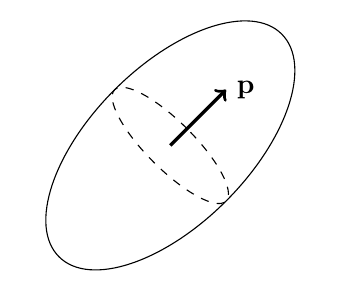
\begin{tikzpicture}[rotate=45]
        \draw(0,0) ellipse (2 cm and 1 cm);
        \draw[dashed](0,0) ellipse (0.3 cm and 1 cm);
        \draw[->,very thick](0,0) --++ (1,0)node[right]{$\textbf{p}$};
    \end{tikzpicture}
    \caption{Scheme of a particle}
    \label{fig:scheme2}
\end{figure}
Let consider a solid axis symmetric particle. 
Due to the axis symmetrical nature of the particle we can stipulate that 
$\mathcal{M}_\alpha =  \textbf{pp}M_{||} +  (\textbf{I} - \textbf{pp})M_\bot$, with $M_{||}$ and $M_\bot$ constant values and \textbf{p} the orientation of the particle see \ref{fig:scheme2}.
Then the internal velocity fields in each particle can be described such as $\textbf{u}_2(\textbf{x}_\alpha + \textbf{r},t) = \textbf{u}_\alpha + \mathbf{\Omega}\cdot \textbf{r}$ where $\Omega$ is the rotation tensor of the particle $\alpha$.
It can be defined as $\mathbf{\Omega}  = \frac{1}{2}\left(\nablabh\textbf{u}_2 - \nablabh\textbf{u}_2^T\right)$ where the gradients are evaluated at $\textbf{y}_\alpha$. 
Meaning that $\textbf{w}_2 = \mathbf{\Omega}\cdot \textbf{r}$.
As a consequence it is easy to show the following relation, $\mathcal{P}_\alpha = \mathcal{M}_\alpha \cdot \mathbf{\Omega}$.
Therefore, from the second moment of mass conservation equation it yields,
\begin{equation}
    \ddt \mathcal{M}_\alpha 
    = \mathcal{M}_\alpha \cdot \mathbf{\Omega} + \mathbf{\Omega} \cdot \mathcal{M}_\alpha.
    \label{eq:dt_M_alpha}
\end{equation}
Then injecting the expression of $\mathcal{M}_\alpha$ in \ref{eq:dt_M_alpha} and  simplifying gives, 
\begin{equation}
    \ddt \textbf{pp} 
    = \mathbf{\Omega} \cdot \textbf{pp} +(\mathbf{\Omega} \cdot \textbf{pp})^T,
    \label{eq:dt_pp_alpha}
\end{equation}
It is interesting to notice that for $M_{||} = M_{\bot}$ \textbf{p} is undefined, and Therefore this equation isn't valid anymore. 
Then, by making use of the moment of momentum conservation equation we have obtain, 
\begin{equation}
    \ddt \left(
        \mathbf{\Omega}\cdot
        \mathcal{M}_\alpha
    \right)
    = \mathbf{\Omega}\mathbf{\Omega} : \mathcal{M}_\alpha + \int \textbf{rT}_1\cdot \textbf{n}_2 d\Sigma
\end{equation}
using the product rule on the LHS together with \ref{eq:dt_M_alpha} yields, 
\begin{equation}
    \ddt 
    \mathbf{\Omega}\cdot
    \mathcal{M}_\alpha
    = 
    - \mathbf{\Omega}\mathcal{M}_\alpha: \mathbf{\Omega}
    + \int \textbf{rT}_1\cdot \textbf{n}_2 d\Sigma
\end{equation}
In agreement with \cite{goldstein2002classical}. 
Then, multiplying this equation by $\mathcal{M}_\alpha^{-1}$, which always exist due to the symmetrical aspect of $\mathcal{M}_\alpha$, we get, 
\begin{equation}
    \ddt 
    \mathbf{\Omega}
    = 
    - \mathbf{\Omega}\cdot \mathbf{\Omega}
    + \int \textbf{rT}_1\cdot \textbf{n}_2 d\Sigma \cdot \mathcal{M}_\alpha^{-1}
\end{equation}
Now  that we got this rather simple equation  


Then, 
